\documentclass[a4paper,11pt,fleqn]{article}%fleqn pour aligner les equations à gauche
\usepackage{../../Styles/Cours}

\newcommand{\chnum}{Chapitre 14}
\newcommand{\chtitle}{Émission et perception d'un son}
\newcommand{\dtype}{TP}

\begin{document}
\maketitle

\section{Les sons et leur propagation}
Un son est créé par la vibration rapide d’un objet (cordes de guitare, ailes d’un insecte, peau frappée …). Cette vibration est souvent d’amplitude faible de l’ordre du micromètre au millimètre entraînant la formation d’un son de faible intensité. Il est donc nécessaire d’amplifier cette vibration grâce à une caisse de résonance.\\
Exemples : caisse de résonance d’une guitare, corps d’un criquet.
	\subsection{La propagation du son}
	Un son est perçu à distance de la source qui l’émet (distance séparant la source sonore de l’oreille). La vibration est donc transmise de proche en proche sans que la source n’ait à se déplacer. Un signal sonore est donc un phénomène de déplacement d’une perturbation de proche en proche dans un milieu matériel et sans transport effectif de matière.\\
Il est donc nécessaire à une onde pour se propager de disposer d’un milieu matériel (exemple : air, bois, métal, eau ou tout autre matériau). En l’absence d’un milieu matériel, il ne peut pas y avoir propagation du son.
	\subsection{Vitesse de propagation du son : la célérité}
	La vitesse du son dans un milieu donné est caractéristique du milieu. Cette célérité dépend de la nature du milieu et de la température. Dans l’air, vers 20°C, la célérité du son est proche de \SI{340}{\meter \per \second}.
    \begin{table}[h!]
        \centering
        \begin{tabular}{|>{\centering}m{3.4cm}|>{\centering}m{3.4cm}|>{\centering}m{3.4cm}|>{\centering}m{3.4cm}|>{\centering \arraybackslash}m{3.4cm}|}
	\hline
	Milieu & Air & Eau liquide & Verre & Acier \\
	\hline
	$v$ ($m.s^{-1}$) & 340 & 1500 & 5300 & 5800 \\
	\hline
	\end{tabular}
        \label{tab:my_label}
    \end{table}
	
\textbf{Exercice d’application :}\\
On place les deux enceintes d’une radio devant deux milieux différents, un aquarium de 15 m de long et un bloc de verre de mêmes dimensions. Quel écart de temps va séparer la perception du son à l’autre bout de l’aquarium et du bloc de verre ?

\begin{table}[h!]
    \centering
    \begin{tabular}{ccccc}
        $v_{eau} = \dfrac{d}{\Delta t}$ & donc & $\Delta t = \dfrac{d}{v_{eau}}$ & $= \dfrac{15}{1500}$ & = \num{0,01} \unit{\second}\\
        $v_{verre} = \dfrac{d}{\Delta t}$ & donc &$\Delta t = \dfrac{d}{v_{verre}}$ & $= \dfrac{15}{5300}$& = \num{0,003} \unit{\second}\\
    \end{tabular}
    \label{tab:my_label}
\end{table}


Le son propagé dans le verre arrivera avant celui propagé dans l'eau. Le retard peut se calculer comme : $retard = \Delta t_{eau} - \Delta t_{verre} = 10 - 7 $ = \num{7} \unit{\milli\second}.

\section{Description d'un signal sonore}
	\subsection{Représentation temporelle}
	Avec un système d’acquisition, on peut visualiser la représentation temporelle d’un signal sonore.
Lorsque la représentation temporelle correspond à la répétition d’un motif élémentaire, on dit qu’elle est périodique.

\begin{figure}
    \centering
    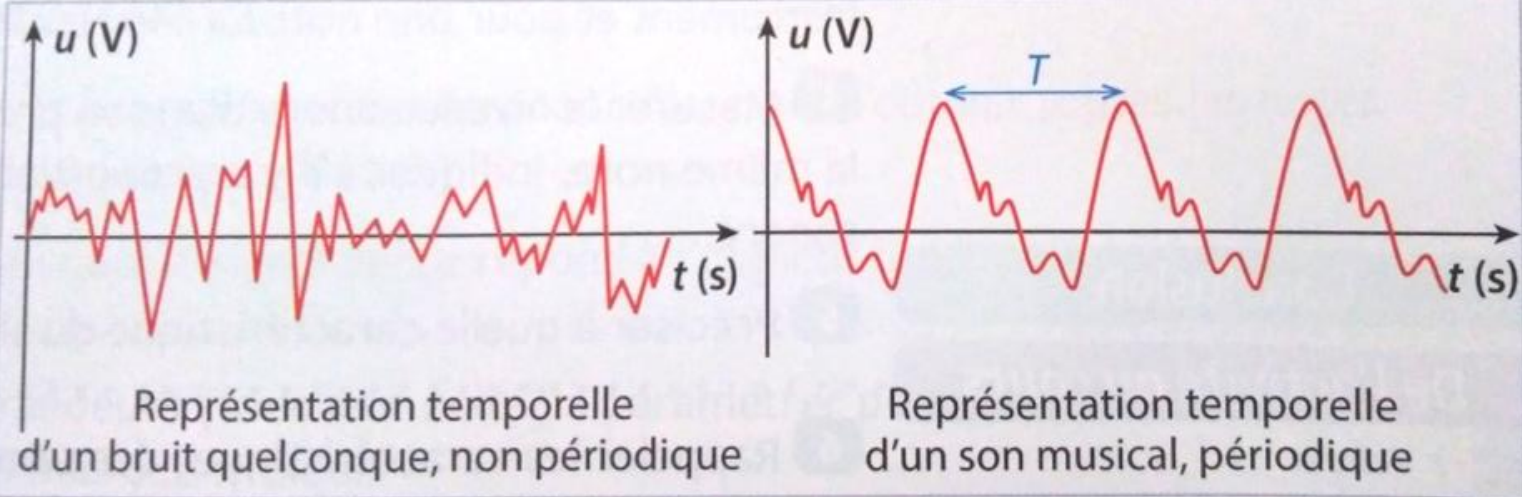
\includegraphics[scale = .3]{Ressources/2GT_C7_Fig1.png}
    \label{fig:my_label}
\end{figure}

	\subsection{Période et fréquence d'un signal sonore}
	La période T d’un signal est la durée en seconde (s) d’un motif élémentaire.
La fréquence f du signal correspond au nombre de répétitions du motif élémentaire par seconde.
$$f=\frac{1}{T}$$
Avec $f$, la fréquence en hertz (Hz) et $T$ la période en (s).
\section{Perception d'un son}
	\subsection{Domaine de fréquence}
	L’oreille humaine permet de dissocier les sons en fonction de leur fréquence. Elle ne peut entendre que les signaux sonores dont les fréquences dont comprises entre 20Hz et 20kHz.
	\begin{figure}[h!]
		\centering
		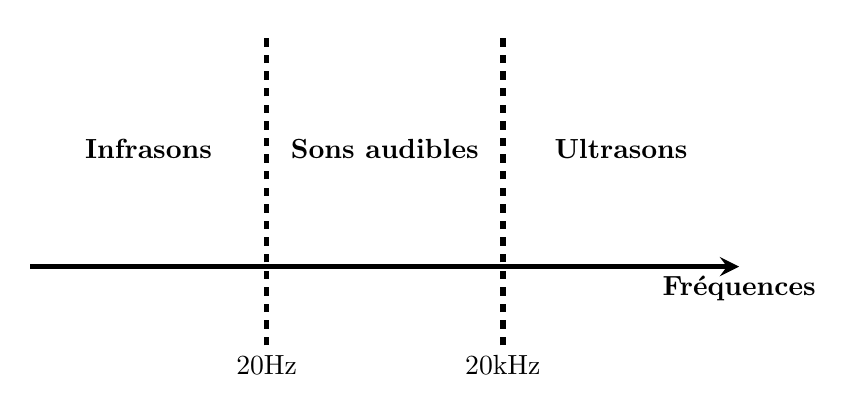
\begin{tikzpicture}
		\draw[line width =2pt,-stealth] (0,0) to (9,0); 
		\draw[dashed, line width = 2pt] (3,-1)--(3,3);
		\draw[dashed, line width = 2pt] (6,-1)--(6,3);
		\node[below] at (3,-1) {\SI{20}{Hz}};
		\node[below] at (6,-1) {\SI{20}{kHz}};
		\node at (1.5,1.5) {\textbf{Infrasons}};
		\node at (4.5,1.5) {\textbf{Sons audibles}};
		\node at (7.5,1.5) {\textbf{Ultrasons}};
		\node[below] at (9,0) {\textbf{Fréquences}};
		\end{tikzpicture}
	\end{figure}
	\subsection{Hauteur d'un son}
	Les sons émis par deux cordes différentes d’un violon ou deux touches d’un piano n’ont pas la même fréquence. Ils n’ont pas la même hauteur.
La hauteur d’un son est la perception auditive procurée par son audition : plus la hauteur d’un son est aiguë, plus sa fréquence est élevée.
Le timbre d’un son est quant à lui lié à la forme du signal sonore.
	\subsection{Intensité et niveau d'intensité sonore}
	Plus l’amplitude d’un signal sonore est élevée, plus l’intensité sonore I est grande. L’intensité sonore s’exprime en watt par mètre carré (\unit{\watt\per\meter\squared})
Pour lier la sensibilité de l’oreille humaine à l’intensité d’un son, le niveau d’intensité sonore ($L$) exprimée en (dB) a été mise en place. Il s’agit de changer d’échelle.
Le niveau d’intensité sonore se mesure à l’aide d’un sonomètre :
\begin{figure}[h!]
		\centering
		\begin{tikzpicture}
		\draw[line width =2pt,-stealth] (0,-.5) to (0,9); 
		\foreach \x in {0,1,...,8}{
		\draw[line width = 2pt] (-.2,\x)--(.2,\x);
		\pgfmathsetmacro{\CalL}{\x};
		\pgfmathsetmacro{\CalI}{\x*10};
		\node[left,color = red!60!black] at (-.2,\x) {$10^\x$};
		\node[right,color = green!60!black] at (.2,\x) {\num[round-mode=places,round-precision=0]{\CalI}};
		}
		\node[left, color= red!60!black] at (-1,9) {\textbf{Intensité sonore $\mathbf{I}$ (\unit{\watt\per\meter\squared})}};
		\node[right, color= green!60!black] at (1,9) {\textbf{Niveau d'intensité sonore $\mathbf{L}$ (\unit{\deci\bel})}};
		\end{tikzpicture}
	\end{figure}
	\subsection{Exposition sonore}
	Les risques liés à l’exposition sonore sont directement liés au niveau sonore et à la durée d’exposition. Une exposition sonore trop élevée peut avoir des conséquences irréversibles, comme une surdité partielle, voir totale.
	\begin{figure}[h!]
	\centering
	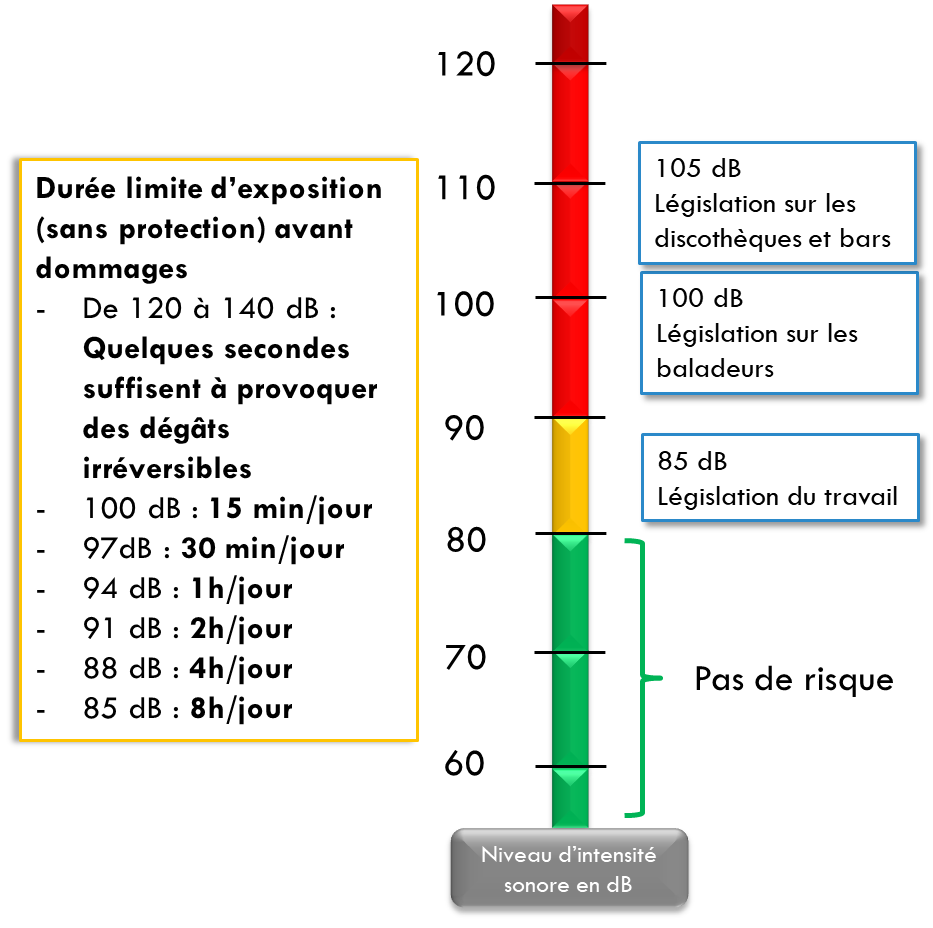
\includegraphics[scale=.4]{Ressources/2GT_C7_Fig2.png}
	\end{figure}
\end{document}